\begin{figure}[b]
  \centering
  \begin{subfigure}{0.5\textwidth} %{{{
    \begin{tikzpicture}[scale=0.8]
      \draw[very thick, ->] (0,0) -- (3.8,0) node[anchor=north] {x};
        % (0,0) node[anchor=north] {0} -- (3.8,0) node[anchor=north] {x};
      \draw[very thick, ->] (0,0) -- (0,3.3) node[anchor=east] {y};
        % (0,0) node[anchor=east] {0} -- (0,3.3) node[anchor=east] {y};
      % first system
      \draw[red, local bounding box=S1, thick]
        (1.2,0.2) rectangle (3.7,2.7);
      \node[red]
        at ({$(S1.west)!0.5!(S1.east)$} |- {$(S1.south)!0.12!(S1.north)$})
        {\small System 1};
      % second system
      \draw[blue, local bounding box=S2, thick]
        (0.2,1.2) rectangle (3.2,3.2);
      \node[blue]
        at ({$(S2.west)!0.5!(S2.east)$} |- {$(S2.south)!0.85!(S2.north)$})
        {\small System 2};
    \end{tikzpicture}
    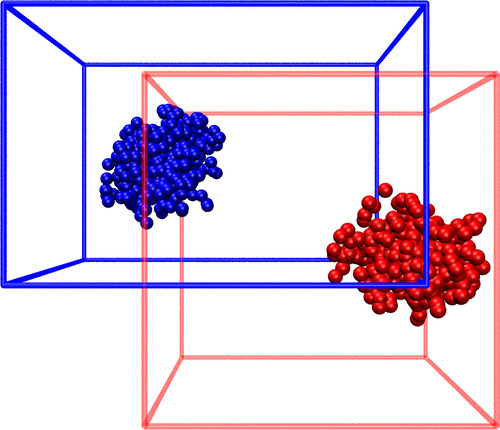
\includegraphics[height=80pt]{JoinSystems-fig_a.jpg}
    \caption{
    } \label{fig:JoinSystems-a}
  \end{subfigure} %}}}

  \begin{subfigure}{0.24\textwidth} %{{{
    \hspace{-13pt}
    \begin{tikzpicture}[scale=0.8]
      \draw[very thick, ->] (0,0) -- (3.8,0) node[anchor=north] {x};
      \draw[very thick, ->] (0,0) -- (0,3.3) node[anchor=east] {y};
      % final system
      \draw[dark-green, local bounding box=new, very thick]
        (0.2, 0.2) rectangle (3.7, 3.2);
      \fill[dark-green!15!white]
        ({$(new.west)$} |- {$(new.north)$}) rectangle
        ({$(new.east)$} |- {$(new.south)$});
      \node[dark-green]
        at ({$(new.west)!0.42!(new.east)$} |- {$(new.south)!0.9!(new.north)$})
        {New System};
      % first system
      \draw[red, local bounding box=S1, dashed, thick]
        (1.2,0.2) rectangle (3.7,2.7);
      \node[red]
        at ({$(S1.west)!0.5!(S1.east)$} |- {$(S1.south)!0.12!(S1.north)$})
        {System 1};
      % second system
      \draw[blue, local bounding box=S2, dashed, thick]
        (0.2,1.2) rectangle (3.2,3.2);
      \node[blue]
        at ({$(S2.west)!0.5!(S2.east)$} |- {$(S2.south)!0.15!(S2.north)$})
        {System 2};
    \end{tikzpicture}

    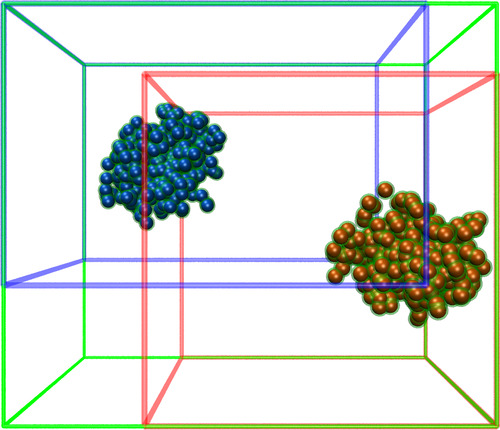
\includegraphics[height=80pt]{JoinSystems-fig_b.jpg}
    \caption{
    } \label{fig:JoinSystems-b}
  \end{subfigure} %}}}
  \begin{subfigure}{0.24\textwidth} %{{{
    \hspace{-13pt}
    \begin{tikzpicture}[scale=0.8]
      \draw[very thick, ->] (0,0) -- (3.8,0) node[anchor=north] {x};
      \draw[very thick, ->] (0,0) -- (0,3.3) node[anchor=east] {y};
      % final system
      \draw[dark-green, local bounding box=new, dashed, thick]
        (0.2, 0.2) rectangle (3.7, 3.2);
      \draw[dark-green, local bounding box=new2, thick]
        (0.95, 0.7) rectangle ++(2.0, 2.0);
      \fill[dark-green!15!white]
        ({$(new2.west)$} |- {$(new2.north)$}) rectangle
        ({$(new2.east)$} |- {$(new2.south)$});
      \draw[dark-green, dashed]
        ({$(new.west)$} |- {$(new.north)$}) --
        ({$(new.east)$} |- {$(new.south)$});
      \draw[dark-green, dashed]
        ({$(new.west)$} |- {$(new.south)$}) --
        ({$(new.east)$} |- {$(new.north)$});
      \draw[dark-green, dashed, very thick]
        ({$(new2.west)$} |- {$(new2.north)$}) --
        ({$(new2.east)$} |- {$(new2.south)$});
      \draw[dark-green, dashed, very thick]
        ({$(new2.west)$} |- {$(new2.south)$}) --
        ({$(new2.east)$} |- {$(new2.north)$});
      % first system
      \draw[red, local bounding box=S1, dashed, thick]
        (1.2,0.2) rectangle (3.7,2.7);
      % second system
      \draw[blue, local bounding box=S2, dashed, thick]
        (0.2,1.2) rectangle (3.2,3.2);
      % \draw[-latex]
      %   ({$(new.west)!0.5!(new.east)$} |- {$(new.north)!0.5!(new.south)$}) --
      %   ({$(new2.west)!0.5!(new2.east)$} |- {$(new2.north)!0.5!(new2.south)$});
      % \node[dark-green]
      %   at ({$(new.west)!0.3!(new.east)$} |- {$(new.south)!1.10!(new.north)$})
      %   {New System};
    \end{tikzpicture}

    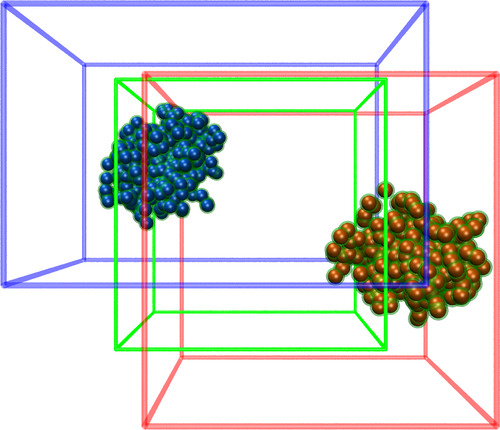
\includegraphics[height=80pt]{JoinSystems-fig_c.jpg}
    \caption{
    } \label{fig:JoinSystems-c}
  \end{subfigure} %}}}
  \begin{subfigure}{0.24\textwidth} %{{{
    \hspace{-13pt}
    \begin{tikzpicture}[scale=0.8]
      \draw[very thick, ->] (0,0) -- (3.8,0) node[anchor=north] {x};
      \draw[very thick, ->] (0,0) -- (0,3.3) node[anchor=east] {y};
      % final system
      \draw[dark-green, local bounding box=new, very thick]
        (0.95, 0.2) rectangle ++(3.0, 2.5);
      \fill[dark-green!15!white]
        ({$(new.west)$} |- {$(new.north)$}) rectangle
        ({$(new.east)$} |- {$(new.south)$});
      \draw[dark-green, dashed, very thick]
        ({$(new.west)$} |- {$(new.north)$}) --
        ({$(new.east)$} |- {$(new.south)$});
      \draw[dark-green, dashed, very thick]
        ({$(new.west)$} |- {$(new.south)$}) --
        ({$(new.east)$} |- {$(new.north)$});
      % first system
      \draw[red, local bounding box=S1, dashed, thick]
        (1.2,0.2) rectangle (3.7,2.7);
      \draw[red, dashed]
        ({$(S1.west)$} |- {$(S1.north)$}) --
        ({$(S1.east)$} |- {$(S1.south)$});
      \draw[red, dashed]
        ({$(S1.west)$} |- {$(S1.south)$}) --
        ({$(S1.east)$} |- {$(S1.north)$});
      % second system
      \draw[blue, local bounding box=S2, dashed, thick]
        (0.2,1.2) rectangle (3.2,3.2);
      \draw[blue, dashed]
        ({$(S2.west)$} |- {$(S2.north)$}) --
        ({$(S2.east)$} |- {$(S2.south)$});
      \draw[blue, dashed]
        ({$(S2.west)$} |- {$(S2.south)$}) --
        ({$(S2.east)$} |- {$(S2.north)$});
      \draw[-latex]
        ({$(S2.west)!0.5!(S2.east)$} |- {$(S2.north)!0.5!(S2.south)$}) --
        ({$(new.west)!0.5!(new.east)$} |- {$(new.north)!0.5!(new.south)$});
      % \node[dark-green]
      %   at ({$(new.west)!0.3!(new.east)$} |- {$(new.south)!1.10!(new.north)$})
      %   {New System};
    \end{tikzpicture}

    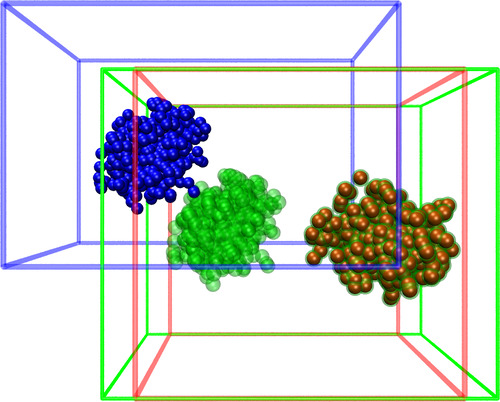
\includegraphics[height=80pt]{JoinSystems-fig_d.jpg}
    \caption{
    } \label{fig:JoinSystems-d}
  \end{subfigure} %}}}
  \begin{subfigure}{0.24\textwidth} %{{{
    \hspace{-13pt}
    \begin{tikzpicture}[scale=0.8]
      \draw[very thick, ->] (0,0) -- (3.8,0) node[anchor=north] {x};
      \draw[very thick, ->] (0,0) -- (0,3.3) node[anchor=east] {y};
      % final system
      \draw[dark-green, local bounding box=new, dashed, thick]
        (0.95, 0.2) rectangle ++(3.0, 2.5);
      \draw[dark-green, local bounding box=new2, very thick]
        (1.45, 0.45) rectangle ++(2.0, 2.0);
      \fill[dark-green!15!white]
        ({$(new2.west)$} |- {$(new2.north)$}) rectangle
        ({$(new2.east)$} |- {$(new2.south)$});
      \draw[dark-green, dashed]
        ({$(new.west)$} |- {$(new.north)$}) --
        ({$(new.east)$} |- {$(new.south)$});
      \draw[dark-green, dashed]
        ({$(new.west)$} |- {$(new.south)$}) --
        ({$(new.east)$} |- {$(new.north)$});
      \draw[dark-green, dashed, very thick]
        ({$(new2.west)$} |- {$(new2.north)$}) --
        ({$(new2.east)$} |- {$(new2.south)$});
      \draw[dark-green, dashed, very thick]
        ({$(new2.west)$} |- {$(new2.south)$}) --
        ({$(new2.east)$} |- {$(new2.north)$});
      % first system
      \draw[red, local bounding box=S1, dashed, thick]
        (1.2,0.2) rectangle (3.7,2.7);
      % second system
      \draw[blue, local bounding box=S2, dashed, thick]
        (0.2,1.2) rectangle (3.2,3.2);
    \end{tikzpicture}

    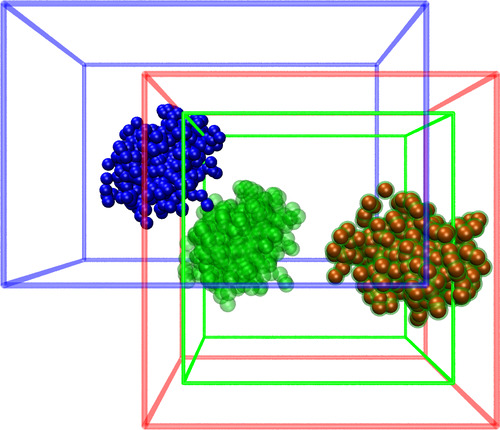
\includegraphics[height=80pt]{JoinSystems-fig_e.jpg}
    \caption{
    } \label{fig:JoinSystems-e}
  \end{subfigure} %}}}
  \caption{
    Schematic representation and corresponding snapshots illustrating
    \tt{JoinSystems} behaviour. (a) The original systems: \tt{System1.lammpstrj}
    (red) and \tt{System2.lammpstrj} (blue) in the \tt{Examples/JoinSystems}
    folder. The rest show examples of possible options (green rectangles and
    transparent balls represent the new systems): (b) no options; (c) \tt{-b 20
    20 20} option; (d) \tt{-off c c c}; (e) \tt{-b 20 20 20 -off c c c}, i.e.,
    combining (c) and (d). These new systems are in the
    \tt{Examples/JoinSystems} folder as \tt{NewSystem\_\#.lammpstrj}, where
    \tt{\#} is \tt{b}, \tt{c}, \tt{d}, or \tt{e}.
  } \label{fig:JoinSystems}
\end{figure}
